\documentclass[main.tex]{subfiles}

\begin{document}
%We will study flows along a network using the tools of linear algebra, revealing interesting parallels with the field of graph theory. In particular, the \emph{Flow Response Transformation}, mapping line flows to the
%We conclude this chapter by deducing a

%\section{Graph}
The power grid forms an interconnected \emph{network} of transmission lines, which makes graph theory a logical choice for modelling it.
In fact, most electrical systems are modelled using graphs. In circuit theory, \emph{lines} represent individual electrical components (resistors, voltage sources) and \emph{nodes} represent the conductive material between them.\footnote{This simplification is only true for components with 2 terminals. A transistor has 3 terminals, for example.}
%More formally, circuit components can be defined as restrictions (boundary conditions) on the \emph{phase space} of the circuit. 
%When we want to create an electric connection between two points, the most obvious way to so is using a \emph{wire}. This has the nice property that 
We will study the electrical properties of the transmission network in Chapter~\ref{chap:model}, but for now, we will simply accept that the transmission network consists of \emph{nodes} and \emph{lines}, and that the lines can transfer power between nodes in a straightforward (linear) way. Physically, the power flows are determined by the amount of power injected at each node, which in turn is determined by the devices that we connect to the transmission network. In this chapter, we will study the \emph{converse}:
\[
\text{\textit{What does the flow of power tell us about the power injection at the nodes?}}
\]
To do so, we will build upon the tools of linear algebra and graph theory, as covered in most elementary textbooks on these subjects.

In this section, we will use, without proof:
\begin{itemize}
\item \emph{Every connected graph contains a minimum spanning tree.}
\item \emph{A connected (di)graph is a \emph{tree} if and only if the number of lines is one fewer than the number of nodes.}
\item \emph{By removing a leaf from a tree, we obtain a new tree.}
\item \emph{Given two nodes in a tree, there is a unique path between these nodes that crosses any line at most once.}
\end{itemize}
\section{Directed graph}
When studying the flow of current in a network, it is necessary to fix a direction for each line, relative to which the flow along that line can be expressed. We do so using a \emph{digraph}, where lines are not defined as two-element sets (like they are in a classical \emph{graph}), but as \emph{ordered pairs}.

\begin{definition}
A \emph{directed graph}\index{graph!directed} is a pair $(\mathcal{N},\mathcal{L})$ such that the set of \emph{nodes} $\mathcal{N}$ is finite, and the set of \emph{lines} $\mathcal{L}\subseteq \mathcal{N} \times \mathcal{N}$ satisfies:
\begin{itemize}
    \item If $(i,j) \in \mathcal{L}$, then $(j,i) \notin \mathcal{L}$. (\ie there are no 'loops' between two nodes.)
    \item For each $i \in \mathcal{N}$: $(i,i) \notin \mathcal{L}$. (\ie no node is directly connected to itself.)
\end{itemize}
\end{definition}

A classical graph can be converted to a \emph{digraph} by (arbitrarily) choosing a direction for each line. Some authors prefer to use a classical graph, combined with an \emph{incidence function}: a function that maps an unordered pair of nodes $\{i,j\}$ to an ordered pair, $(i,j)$ or $(j,i)$.\footnote{\cite{Slepian1968} takes this one step further by \emph{only} considering the incidence function: the set of lines can be retrieved as the \emph{domain} of the incidence function, and the set of nodes is the \emph{union} of the set of lines.}

\section{Flow}
For the remainder of this section, assume that $G=(\mathcal{N},\mathcal{L})$ is a directed graph, where the nodes are labelled $\mathcal{N}=\{1,2,\dots,n\}=\range{n}$ for some $n \in \mathbb{N}$.
The $m = \# \mathcal{L}$ lines of the network are labelled $\mathcal{L}=\{\mathcal{L}_1,\mathcal{L}_2,\dots,\mathcal{L}_m\}$.

We also fix a field $\mathbb{K}$, which we will use to define \emph{injections} and \emph{flows} on $G$. When studying \emph{real power flows}, we will take $\mathbb{K}=\mathbb{R}$.

\begin{definition}\label{def:injectionandflow}
An \define{injection on $G$} is an element of $\mathbb{K}^n$; a \define{flow on $G$} is an element of $\mathbb{K}^m$.
\end{definition}

One should view an injection $\mat{p} \in \mathbb{K}^n$ as the vector that encodes how much power is being put into the network at each node. When $\mel{p}_i$ is negative, this means that power is being \emph{consumed} at node $i$. Similarly, a flow $\mat{f} \in \mathbb{K}^m$ represents the amount of power transmitted along each line. For a line $\mathcal{L}_k=(i,j) \in \mathcal{L}$, $\mel{f}_k$ expressed the amount of power being transmitted along the line, from node $i$ to node $j$.

Of course, the notions \emph{positive} and \emph{negative} only exist when $\mathbb{K}$ is a totally ordered set. Otherwise, we simply have to be satisfied with the meaning provided by Definition~ \ref{def:inducedinjection}.

When $\mathbb{K}=\mathbb{F}_2$, a flow can be seen as a subset of the collection of lines $\mathcal{L}$, since any flow entry is either $1$ or $0$.

\begin{definition}\label{def:inducedinjection}
An injection $\mat{p} \in \mathbb{K}^n$ is \emph{induced}\index{induced injection} by a flow $\mat{f} \in \mathbb{K}^m$ if:
\begin{gather}
    \mel{p}_i =
    \sum_{\mathcal{L}_k=(i,j) \in \mathcal{L}} f_k -
    \sum_{\mathcal{L}_k=(j,i) \in \mathcal{L}} f_k \label{eq:inducedflow}
\end{gather}
for each node $i \in \mathcal{N}$. ($\mel{p}_i = 0$ for isolated nodes.)
\end{definition}
Note that $\mat{p}$ is uniquely defined for every choice of $\mat{f}$. This allows us to define a function:
\begin{definition}
Suppose $G$ has no isolated nodes. We define the \define{Flow Response Transformation} ($\FRT$) as the function
\begin{gather*}
    \FRT: \mathbb{K}^m \rightarrow \mathbb{K}^n
\end{gather*}
that maps a flow $\mat{f} \in \mathbb{K}^m$ to the unique injection $\mat{p} \in \mathbb{K}^n$ that it induces.
\end{definition}

From (\ref{eq:inducedflow}), it follows that $\FRT$ is a linear map, which means that we can write $\FRT$ as a matrix: $\mat{K}$. We can find an explicit expression for the entries $\mel{K}_{i,k}$, noting that its \emph{rows} are determined by (\ref{eq:inducedflow}), and that there are no `double' lines in the digraph.

\begin{align*}
    \mel{K}_{i,k} =
    \begin{cases}
         1 & \text{if } \mathcal{L}_k=(i,j) \text{ for some } j \in \range{n}, \\
        -1 & \text{if } \mathcal{L}_k=(j,i) \text{ for some } j \in \range{n}, \\
         0 & \text{otherwise}.
    \end{cases}
\end{align*}

This matrix can be seen as the familiar \emph{incidence matrix} of a classical graph, adapted to digraphs. For this reason, $\mat{K}$ is often called the \emph{vertex-edge incidence matrix of $G$}.
The ordered set of lines is uniquely defined by the vertex-edge incidence matrix.

\begin{figure}
    \centering
    %\documentclass{standalone}\usepackage{tikz}\begin{document}


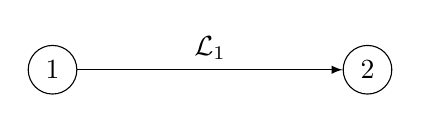
\begin{tikzpicture}

\def \width{4cm}
\def \margin{4mm}

\node (1) [draw, circle] at (0,0) {$1$};
\node (2) [draw, circle] at ({\width},0) {$2$};
\draw[->, >=latex] (1) -- node[above] {$\mathcal{L}_1$} (2);

\end{tikzpicture}


%\end{document}
    \caption{The simple \emph{two-node}\index{network!two-node} network of two nodes and one line.}
    \label{fig:twonodes}
\end{figure}
\begin{example}[Two-node network]\label{exa:twonodenetwork}
A very simple digraph is one with just two nodes, and a single line connecting them. This \emph{two-node network}\index{network!two-node} is drawn in Figure \ref{fig:twonodes}.
Although real networks are much bigger, this example is useful to illustrate some of the concepts introduced in Chapter~\ref{chap:model}.
\begin{align*}
    \intertext{We have:}
    \mathcal{N}&=\{1,2\} \text{ and}\\
    \mathcal{L}&=\{\mathcal{L}_1\}\text{ with }\mathcal{L}_1=(1,2). \\
    \intertext{Since $n=2$ and $m=1$, $\mat{K}$ is a $2\times 1$ matrix:}
    \mat{K} &= \begin{pmatrix}
    1 \\
    -1
    \end{pmatrix}.
\end{align*}
\end{example}

\begin{figure}[h]
    \centering
    %\documentclass{standalone}\usepackage{tikz}\begin{document}


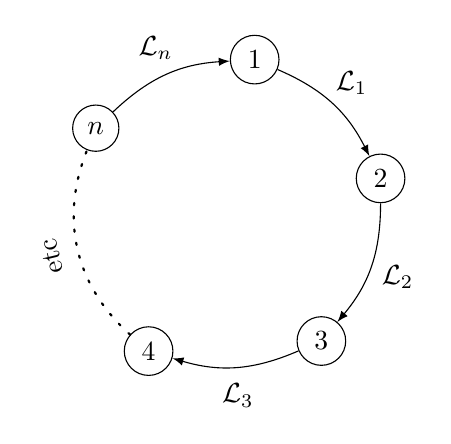
\begin{tikzpicture}

\def \margin{4mm}
\def \radius {2cm}
\def \labelsep {3mm}
\def \dotsep {.4mm}
\def \bend {20}
\def \dotbend {35}
\def \dotmargin {15}

\def \n {4}

\foreach \i in {1,...,\n}
{
  \node (\i) [draw,circle] at ({180 - 360/(\n + 1.4) * (\i +.5)}:\radius) {\i};
}

\foreach \i [remember=\i as \lasti (initially 1)] in {2,...,\n}
{
  \draw[->, >=latex] (\lasti) to[bend left=\bend] (\i);
  \node at ({180 - 360/(\n + 1.4) * (\i +.5 - .5)}:{\radius + \labelsep}) {$\mathcal{L}_\lasti$};
  \node at ({0 + (360/(\n + 1.4) * (\i +.5 - .5))}:{\radius + \labelsep}) {\hphantom{$\mathcal{L}_\lasti$}};
}

\node (n) [draw, circle] at ({180 - 360/(\n + 1.4) * (0 +.5)}:\radius) {$n$};

\draw[->, >=latex] (n) to[bend left=\bend] (1);
\node at ({180 - 360/(\n + 1.4) * (1 +.5 - .5)}:{\radius + \labelsep}) {$\mathcal{L}_n$};

\node[rotate=(( - 360/(\n + 1.4) * (\n/2 + .5)) - 90)] at ({(-360/(\n + 1.4) * (\n/2 + .5))}:{\radius + \labelsep}) {etc};

\draw[thick,line cap=round,loosely dotted, >=latex] (\n) to[bend left=\dotbend] (n);
%\draw[thick,line cap=round,loosely dotted] ({360/(\n + 1.4) * (0 +.5) - \dotmargin}:{\radius - \dotsep}) arc ((360/(\n + 1.4) * (0 +.5))+360 - \dotmargin:(360/(\n + 1.4) * (4 +.5)) + \dotmargin:\radius - \dotsep);


%\draw[color=red] (0:\radius) arc (0:360:\radius);

%\node (1) [draw, circle] at (0,0) {$1$};
%\node (2) [draw, circle] at ({\width},0) {$2$};
%\draw[->, >=latex] (1) -- node[above] {$\mathcal{L}_1$} (2);

\end{tikzpicture}


%\end{document}
    \caption{The \emph{$n$-loop}\index{network!$n$-loop} network with $n$ nodes and $n$ lines.}
    \label{fig:nloopnetwork}
\end{figure}

\begin{example}[Loop network]\label{exa:nloopnetwork}
A less trivial digraph is the \emph{$n$-loop network}\index{network!$n$-loop}, shown in Figure~\ref{fig:nloopnetwork}. It consists of $n$ nodes, connected in a circular fashion (using $n$ lines).

Note that this network is 2-edge connected, meaning that the network remains connected when any edge is removed. (Although removing \emph{any} two lines will disconnect the network.)
\begin{align*}
    \intertext{We have:}
    \mathcal{N}&=\{1,\dots,n\}=\range{n} \text{ and}\\
    \mathcal{L}&=\{\mathcal{L}_1,\dots,\mathcal{L}_n\}\text{ with }\mathcal{L}_i=(i,i+1)\text{ for }1 \leq i < n\text{ and }\mathcal{L}_n=(n,1). \\
    \intertext{Since $m=n$, $\mat{K}$ is an $n\times n$ matrix:}
    \mat{K} &= \begin{pmatrix}
    1 &  & &  & &  -1 \\
    -1 &  1 &  &   &   &   \\
      & -1 &  1 &  &       & \\
      &   &  \ddots & \ddots  &   &   \\
      &   &   & & 1 &    \\
      &   &  &  & -1 &      1  \\
    \end{pmatrix}.
\end{align*}
\emph{(All unspecified elements are 0).}

Note that the \emph{columns} of $\mat{K}$ correspond to the lines of the network.
\end{example}

\begin{figure}
    \centering
    \includegraphics[width=.5\textwidth]{img/scigrid_boring.pdf}
    \caption{The $n=489$ buses and $m=695$ lines of the SciGRID network. A description of this dataset is given in Part II.}
    \label{fig:scigrid}
\end{figure}
\begin{example}[SciGRID Germany]\label{exa:scigridnetwork}
In Part II, we will apply our theory to the SciGRID dataset, which contains the network shown in Figure~\ref{fig:scigrid}. This network is much more realistic than the previous examples, as it is based on the real-world structure of the transmission network in Germany. 

It is common for transmission networks to have a well-connected `core', with some branches out of the core towards the outer regions of the network. This means that in general, $m>n$.

Indeed, in this network we have $n=489$ and $m=695$. The vertex-edge incidence matrix $\mat{K}$ has dimensions $489 \times 695$, and it is \emph{sparse}: most entries are zero.

It is important to note that this is only a \emph{section} of the actual transmission network of continental Europe, which is highly connected among different countries. As we will discuss in Section \ref{sec:constructingdataset}, accurate datasets of continental Europe do exist, but they are hard to obtain and analyse.
%Because the laws of physics have no notion of national borders, we would 
%As far as the laws of physics are concerned, taking the subset of lines within Germany is almost as arbitrary as, say, the subset of lines above a certain latitude.
\end{example}

The fact that $\FRT$ is a linear map raises an interesting question: how can the image and kernel of $\FRT$ be interpreted in the context of digraph flows?
The reader is invited to revisit Example \ref{exa:nloopnetwork} to visualise these sets.

One can interpret the image of $\FRT$ as the set of injections that can be redistributed along the network. Because a flow only serves to redistribute injections from one node to another, nothing is lost or gained in the network. This imposes the condition that an injection vector must have \emph{zero sum}. Moreover, when $G$ is connected, \emph{all} zero sum injections can be induced by a flow.

The kernel can be interpreted as the set of all flows that result in zero injections. Besides the trivial case of zero flow, any constant flow along a loop induces zero injection. We will find that these \emph{loop flows} generate \emph{all} flows in the kernel of $\FRT$.

When $G$ is a planar graph, loops around the faces of $G$ actually form a \emph{basis} for the kernel. In the more general case that $G$ is connected, but not necessarily planar, such a basis can also be constructed by fixing a \emph{minimum spanning tree} of $G$.

As an added bonus, applying the Rank-Nullity theorem to $\FRT$ when $G$ is planar provides us with an alternative demonstration of Euler's Formula.

These statements will be made more precise in the next sections, when we study the image and kernel of $\FRT$ in more detail.

\section{Image of $\mathbf{\FRT}$}
We start with the following definition:
\begin{definition}
The function $\sigma : \mathbb{K}^n \rightarrow \mathbb{K}$ defined by
\begin{gather*}
    \sigma : \mat{p} \mapsto \sum_{i=1}^n \mel{p}_i
\end{gather*}
is the linear map from an injection vector $\mat{p}$ to the \define{net injection} of $\mat{p}$.
\end{definition}
The kernel of $\sigma$ is the set of zero-sum injections:
$$\ker \sigma = \left\{ \mat{p} \in \mathbb{K}^n \, \mid \, \sum_{i=1}^n \mel{p}_i = 0 \right\}.$$
When $G$ is connected, this is exactly the set of injections that can be induced by a flow on $G$:

\begin{theorem}\label{thm:imageLPF}
Suppose that $G$ is connected. Then
\begin{empheq}[box=\fbox]{gather}
    \Ima \FRT = \left\{ \mat{p} \in \mathbb{K}^n \, \mid \, \sum_{i=1}^n \mel{p}_i = 0 \right\} \cong \mathbb{K}^{n-1}
\end{empheq}
\end{theorem}

We will prove this equality by considering the two inclusions $\subseteq$ and $\supseteq$ separately. The first inclusion follows from the observation that $\mat{K}$ is the vertex-edge incidence matrix of $G$.
\begin{lemma}\label{lem:imlpfsubsetkersigma}
Suppose that $G$ is connected.
\begin{gather}
\Ima \FRT \subseteq \ker \sigma\label{eq:LPFfin}
\end{gather}
\end{lemma}
\begin{proof}
We write $\mat{e}^1, \dots, \mat{e}^m$ for the standard basis of $\mathbb{K}^m$.

Since $\FRT$ is linear, one only needs to verify that $\FRT(\mat{f}) \in \ker \sigma$ for each $\mat{f}=\mat{e}^k$ in the basis.
The vectors $\FRT(\mat{e}^1), \dots, \FRT(\mat{e}^m)$ are exactly the columns of the matrix $\mat{K}$, which all have zero sum: a column corresponds to a line in $G$, and has exactly two non-zero entries: $1$ for the entering node, and $-1$ for the leaving node.
\end{proof}

To prove the inclusion $\supseteq$ implied by Theorem \ref{thm:imageLPF}, we first consider the special case that $G$ is a \emph{tree}.

\begin{lemma}\label{lem:connectedtree}
Suppose that $G$ is a (connected) tree.
\begin{gather}
\Ima \FRT \supseteq \ker \sigma
\end{gather}
\end{lemma}

\begin{proof}%\todo{This proof could benefit from an illustration.}
$G$ is a tree, so $m=n-1$. Because $\mathbb{K}^m$ and $\ker \sigma$ both have dimension $n-1$, we only need to prove that $\FRT$ is injective: when $\FRT$ has nullity $0$, it must have rank $n-1$.

If $n=1$, then the digraph consist of a single node, and no lines. It then follows from (\ref{eq:inducedflow}) that the only injection that can be induced is $\mat{p}=(0) \in \mathbb{K}^1$, so $\FRT$ can only be injective.

If $n>1$, we will use the fact that the statement holds for any tree with fewer than $n$ nodes. \emph{(Proof by induction.)}

Suppose that $f \in \mathbb{K}^{m}$, such that $\mat{p}=\FRT(\mat{f})=\mat{0}$. Because $G$ is a tree, we can\footnote{Write $\gr(i)$ for the number of lines connected to $i$. $G$ is connected, so $\gr(i)\geq1$ for each $i \in \mathcal{N}$. \emph{If no $i$ exists with $\gr(i)=1$}, then $\gr(i)\geq 2$ for each $i \in \mathcal{N}$, giving $\sum_{i = 1}^n \gr(i) \geq 2n$. On the other hand, each of the $n-1$ lines connects exactly two nodes, so $\sum_{i = 1}^n \gr(i) = 2(n-1) < 2n$, a contradiction.} pick a \emph{leaf} $i \in \mathcal{N}$, which has a unique line $\mathcal{L}_k$ connecting $i$ to some $j \in \mathcal{N}$. (We have either $\mathcal{L}_k = (i,j)$ or $\mathcal{L}_k=(j,i)$.)

Only one line is connected to $i$, so (\ref{eq:inducedflow}) gives: $\mel{p}_i = \pm \mel{f}_k$. (The sign depends on the orientation of $\mathcal{L}_k$.) We assumed $\mel{p}_i=0$, so we must have $f_k = 0$.

By removing node $i$ and line $\mathcal{L}_k$, we obtain a smaller tree, for which the statement already holds. The Flow Response Transformation of this subtree is essentially the restriction of $\FRT$ to the set $\left\{\mat{f} \in \mathbb{K}^m \, \mid \, \mel{f}_k = 0\right\}$. Because the restriction is injective, all other coefficients of $\mat{p}$ are also zero. This shows that $\FRT$ is injective, and the result follows.
\end{proof}

\begin{proof}[Proof of Theorem \ref{thm:imageLPF}]
To prove $\Ima \FRT = \ker \sigma$, it remains to show that
\begin{gather}
\Ima \FRT \supseteq \ker \sigma
\end{gather}
holds for \emph{any} connected $G$, not just for trees.

Since $G$ is connected, we can choose a minimum spanning tree: choose $T \subseteq \range{m}$ with $\# T = n-1$ such that $G_T=(\mathcal{N}, \{\mathcal{L}_k\}_{k \in T})$ is such a connected subdigraph.

Define $F_T = \linspan \{\mat{e}^k\}_{k \in T} \subseteq \mathbb{K}^m$ as the subset of flows on $G$ that are zero outside of $G_T$. Because $F_T$ is a linear subspace of $\mathbb{K}^m$, we have
$$\Ima \FRT = \FRT (\mathbb{K}^m) \supseteq \FRT(F_T),$$
which reduces the problem to $\FRT(F_T) \supseteq \ker \sigma$, which follows from Lemma \ref{lem:connectedtree}.

This shows that
\begin{gather*}
    \Ima \FRT = \ker \sigma.
\end{gather*}
Because $\sigma : \mathbb{K}^n \rightarrow \mathbb{K}$ is surjective, it has rank $1$. It therefore has nullity $n-1$, or equivalently, $\ker \sigma \cong \mathbb{K}^{n-1}$.
\end{proof}









\section{Kernel of $\mathbf{\FRT}$}
Again, let us assume that $G$ is connected. In Theorem \ref{thm:imageLPF}, we derived an explicit formulation for the image of $\FRT$, showing that $\rank \FRT = n-1$.

Concerning the kernel of $\FRT$, we already know that $\mat{0} \in \ker \FRT$, reflecting the fact that zero flow induces zero injection. In the special case that $G$ is a tree, this is the only such flow. In general, however, the kernel of $\FRT$ is much bigger.

\begin{proposition}\label{prop:nullityLPF}
Suppose that $G$ is connected. The dimension of $\ker \FRT$ equals
\begin{gather*}
    \nullity \FRT = m - (n - 1).
\end{gather*}
\end{proposition}
\begin{proof}
This follows directly from the Rank-Nullity theorem, applied to Theorem \ref{thm:imageLPF}.
\end{proof}


\begin{corollary}
If $G$ is a tree, then $\ker \FRT = \{\mat{0}\}$, and $\FRT$ is an isomorphism between $\mathbb{K}^m$ and $\ker \sigma$.
\end{corollary}
\begin{proof}
Applying Proposition \ref{prop:nullityLPF} with $m = n-1$, we find that $\nullity \FRT = 0$, so that ${\ker \FRT = \{\mat{0}\}}$. Together with Theorem \ref{thm:imageLPF}, we find the result.
\end{proof}

\subsection{Loop flows}
What do the elements of $\ker \FRT$ look like? As we will see, any flow along a \emph{loop}\footnote{We define a \emph{path} by the ordered sequence of nodes that it visits, including the initial and final node. Although we are studying directed graphs, lines can be traversed in either direction by a path. A \emph{loop} is a path where the initial and final node coincide.} results in zero power injection. When interpreting a loop as an element $\mat{f}$ of $\mathbb{K}^m$, we must be careful to \emph{flip the sign of $\mel{f}_k$ if the line $\mathcal{L}_k$ is traversed in reverse.}

\begin{theorem}\label{thm:loopflowkernel}
Suppose that $G$ is connected and that $(i_1, i_2, \dots, i_p)$ is a loop that visits each line at most once. Then the \define{loop flow} $\mat{f} \in \mathbb{K}^m$ defined by:
\begin{gather}
    \mel{f}_k = \begin{cases}
    \hphantom{-}1 & \text{if } (i_s\hphantom{_{+1}}, i_{s+1})=\mathcal{L}_k \text{ for any } 1 \leq s < p,\\
    -1 & \text{if } (i_{s+1}, i_s\hphantom{_{+1}})=\mathcal{L}_k \text{ for any } 1 \leq s < p,\\
    \hphantom{-}0 & \text{otherwise,}
    \end{cases}\label{eq:loopflowdef}
\end{gather}
for each line $\mathcal{L}_k$, is an element of the kernel of $\FRT$.
\end{theorem}
\begin{proof}
We will verify that $\mat{p}=\FRT(\mat{f})$ is zero.
Choose any $i \in \mathcal{N}$.

Because the loop is closed, there is an \emph{even} number (possibly zero) of lines with non-zero flow that connect to $i$. This means that the sums in (\ref{eq:inducedflow}) cancel each other (note the negative sign for reversed lines in (\ref{eq:loopflowdef})), resulting in $\mel{p}_i=0$.
\end{proof}

\begin{remark}
Because $\FRT$ is linear, multiplying a loop flow with a scalar $\gamma \in \mathbb{K}$, or adding two loop flows, creates a new flow that induces zero injection. (The result of addition is a flow, but in general not a \emph{loop} flow.)
\end{remark}

Now that we know the dimension of $\ker \FRT$, a natural next step is to look for a \emph{basis} that generates the kernel. Motivated by the previous theorem, we will look for a basis consisting of \emph{loop flows}.

A logical choice for this basis would be the set of all flows in \emph{loops surrounding the faces contained in the graph}. This approach, which only works for \emph{planar graphs}, will be discussed in the next section.

For now, we would like to find a basis of loop flows for the more general case that $G$ is connected, but not necessarily planar. We proceed as follows:

\begin{definition}\label{def:spiderwebbasis}
Suppose that $G$ is connected, and that $T \subseteq \range{m}$ is a minimum spanning tree. For each remaining line $\mathcal{L}_k = (i,j) \in \left\lbrace \mathcal{L}_k \in \mathcal{L} \, \mid \, k \notin  T \right\rbrace $, there exists a \emph{unique path along the tree} from $j$ to $i$ that crossed any line at most once, say 
\[
(i_1, i_2, \dots, i_p),\quad\text{ where $i_1=j$ and $i_p=i$.}
\]
By adding the chosen line $\mathcal{L}_k$ to this path, we find a loop in $G$: $(i_1, i_2, \dots, i_p, j)$, which defines a loop flow $\mat{f}^k$. 

We define the \define{spider web basis on $T$} as the set of loop flows defined this way: $\{ \mat{f}^k \}_{k \in \range{m} \setminus T}$. (If $T$ were to represent a physical tree, a spider could spin a web from $i$ to $j$ by attaching a strand to $j$ and then walking the path to $i$.\footnote{It turns out that this is not how most spiders cover large distances: instead, they produce a long thread, and let it drift in the wind until it sticks to another surface. Clever!})
\end{definition}

\begin{theorem}
The \emph{spider web basis on $T$} constructed in Definition \ref{def:spiderwebbasis} is a basis for $\ker \FRT$.
\end{theorem}
\begin{proof}
Because $T$ is a minimum spanning tree, it has $n-1$ elements, and so the spider web basis consists of $m - (n-1)$ loop flows.
Because the number of elements in the basis equals the dimension of $\ker \FRT$, one only needs to prove that they are linearly independent. Indeed, for each $k \in \range{m}\setminus T$, the loop flow $\mat{f}^k$ is the only element for which the $k^{\text{th}}$ entry is non-zero. Therefore, $\mat{f}^k$ cannot be written as linear combination of the other fundamental loops.
\end{proof}

\subsection{Planar Graphs}
The spider web basis can be constructed for any connected graph. When the graph is also \emph{planar}, a more intuitive basis exists. Without providing a rigorous definition, we simply say that a graph is \define{planar} if it can be `drawn on a piece of paper without any crossing lines'. Such a drawing creates \emph{faces}: areas enclosed by lines.\footnote{We do not consider the infinite enclosing area as one of the faces.} Different drawings can produce different collections of faces.

If we fix a collection of faces for a planar graph, then each face is enclosed by some of the lines, which form a loop in the graph. We define the \emph{planar basis on this drawing} as the set of loop flows defined by those loops: each face becomes an element in the basis. Rewriting Theorem~\ref{prop:nullityLPF}, we find:
%
%\towrite{th: in a planar embedding of a planar graph, the loops surrounding faces form a basis.
%proof: (in F2): 
%
%linearly independent: these loops are all loops with the property that exactly one face is contained in the loop.
%
%complete: start with a spider web basis.
%choose a loop f in the spider web basis.
%this loop f contains a number of faces. f is equal to the sum of the loops around these faces.
%this shows that f can be written as linear combination of planar loops. QED}

\begin{corollary}[Euler's Formula]
In a planar, connected graph, we have:
$$v + f - e = 1$$
where $v$ is the number of vertices, $e$ is the number of edges, and $f$ is the number of faces enclosed by edges, excluding the 'exterior face'.
\end{corollary}
\end{document}
